 \documentclass[12pt]{article}
\usepackage[T2A]{fontenc}
\usepackage[utf8]{inputenc}       

\usepackage[english]{babel}
\usepackage{amsmath,amsfonts,amsthm,amssymb,amsbsy,amstext,amscd,amsxtra,multicol}
\usepackage{verbatim}
\usepackage{tikz}
\usetikzlibrary{automata,positioning}
\usepackage{multicol}
\usepackage{graphicx}
\usepackage[colorlinks,urlcolor=blue]{hyperref}
\usepackage[stable]{footmisc}
\usepackage{ dsfont }
\usepackage{wrapfig}
\usepackage{xparse}
\usepackage{ifthen}
\usepackage{bm}
\usepackage{color}
 \usepackage{subfigure}
 
\usepackage{algorithm}
\usepackage{algpseudocode}

\usepackage{xcolor}
\usepackage{hyperref}
\definecolor{linkcolor}{HTML}{799B03} % цвет гиперссылок
\definecolor{urlcolor}{HTML}{799B03} % цвет гиперссылок
 
%\hypersetup{pdfstartview=FitH,  linkcolor=linkcolor,urlcolor=urlcolor, colorlinks=true}

\newtheorem{theorem}{Theorem}[section]
\newtheorem{lemma}{Lemma}[section]

\DeclareMathOperator{\sign}{sign}
\DeclareMathOperator{\grad}{grad}
\DeclareMathOperator{\intt}{int}
\DeclareMathOperator{\conv}{conv}
\begin{document}

\section{Данные}

В собранной коллекции имелось 100 пар текстов. Каждая пара состоит из написанного в спокойном состоянии и написанного в фустрированном состоянии одним и тем же человеком текстов. Для каждого текста были вычислены одинаковые признаки (всего призноков 198), и для каждой пары была вычислена разница между текстами и была предпринята попытка кластеризации пар по этой разнице.

Пусть $F$ - матрица объект признак для текстов, написанных в фустрированном состоянии, $C$ - матрица объект признак для текстов, написанных в спокойном состоянии, тогда $D = F-C$ - матрица объект-признак для пары текстов. Далее мы будем говорить о нормализованных данных.

\section{Кластеризация}
\label{sec:cluster}

\begin{figure}[h!]
\center{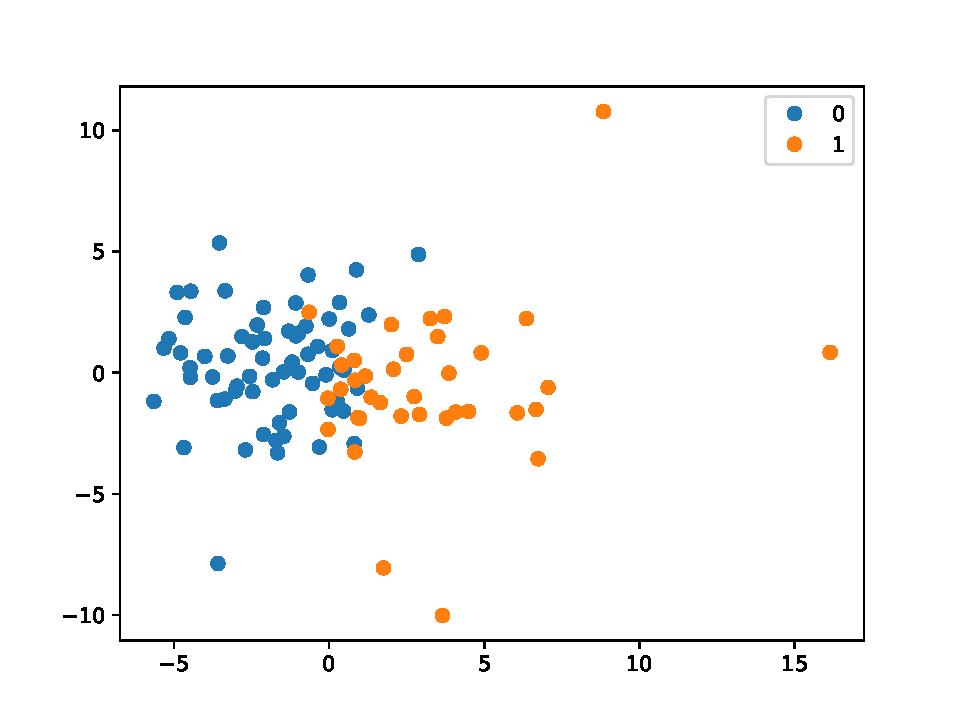
\includegraphics[scale=0.8]{Images/Cluster.pdf}}
\label{cluster}
 \caption{Кластеризация на два класса: визуализация при помощи PCA}
\end{figure}

Используя различные методы визуализации, в частности, PCA, можно увидеть, что данные представляют собой достаточно непрерывное единое облако точек с небольшими выбросами.

Были опробованы различные методы кластеризации. Было решено остановиться на KMeans с предварительным снижением размерности при помощи метода PCA до 10. Результат кластеризации на два кластера Вы можете видеть на рисунке \ref{cluster}. Как можно видеть, подобная кластеризация просто разрезает вышеупомянутое облако точек приблизительно по центру.

Классы получаются достаточно сбалансированными и при трех кластерах. При большом количестве кластеров получаемое разбиение по большей части просто отсеивает крайние точки.

\section{Основные Различия Между Кластерами}

Далее выделим главные отличия между двумя кластерами, полученными в прошлом разделе. Сначала определим по каким признакам эти кластеры различаются больше всего. Для этого для каждого признака посчитаем квадрат разности между его средним значением по первому кластеру и по второму. Получим, что приблизительно для 120 признаков эта разница околонулевая. Пусть $M$ - максимальная разница между признаками, тогда возьмем все признаки для которых разница лежит в диапазоне от $[0.7M, M]$. Всего таких признаков получили шесть. Их наименования в порядке возрастания разницы:

\begin{itemize}
\item Доля глаголов прошедшего времени, первого лица, единственного числа
\item Часть речи: прилагательное
\item Часть речи: существительное
\item Средняя длина слов (в количестве символов)
\item Коэффициент Трейгера
\item Часть речи: местоимение-существительное
\end{itemize}

Посмотрим на распределения для соответствующих признаков. Для каждого признака мы взяли интервал, в котором лежат значения этого признака, разбили его на 10 частей, посчитали для каждого кластера количество объектов со значением этого признака в соответствующей части и нормализовали полученные данные (сделали так, чтобы интеграл по всему интервалу был равен единице). Соответствующие гистограммы Вы можете видеть на \ref{hist}.

\begin{figure}[ht!]  
\vspace{-4ex} \centering \subfigure[]{
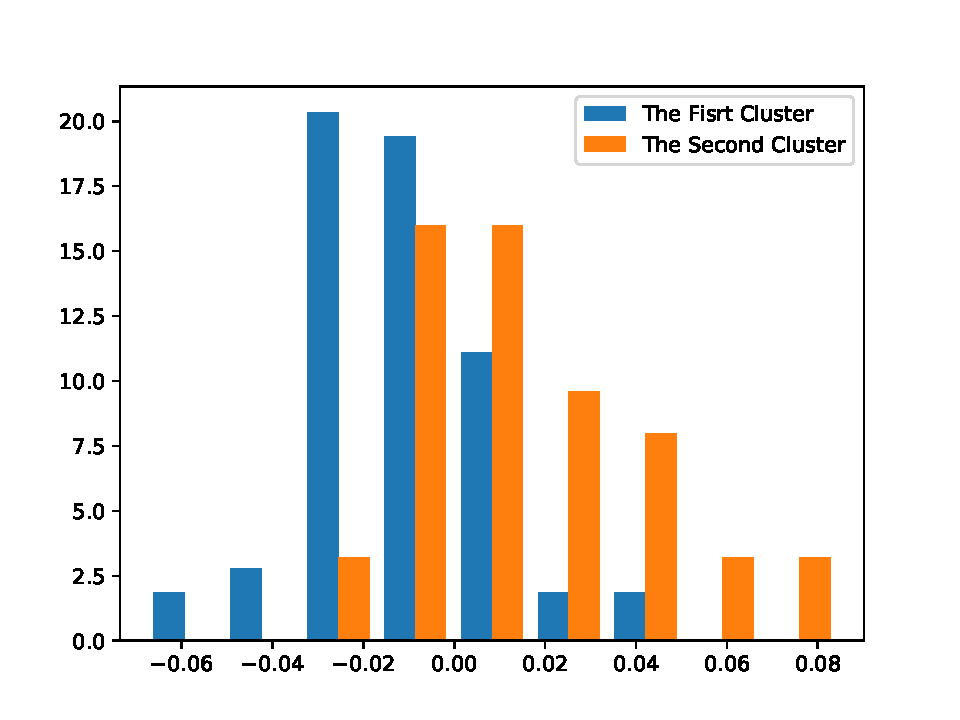
\includegraphics[width=0.4\linewidth]{Images/1.pdf} \label{1} }  
\hspace{2ex}
\subfigure[]{
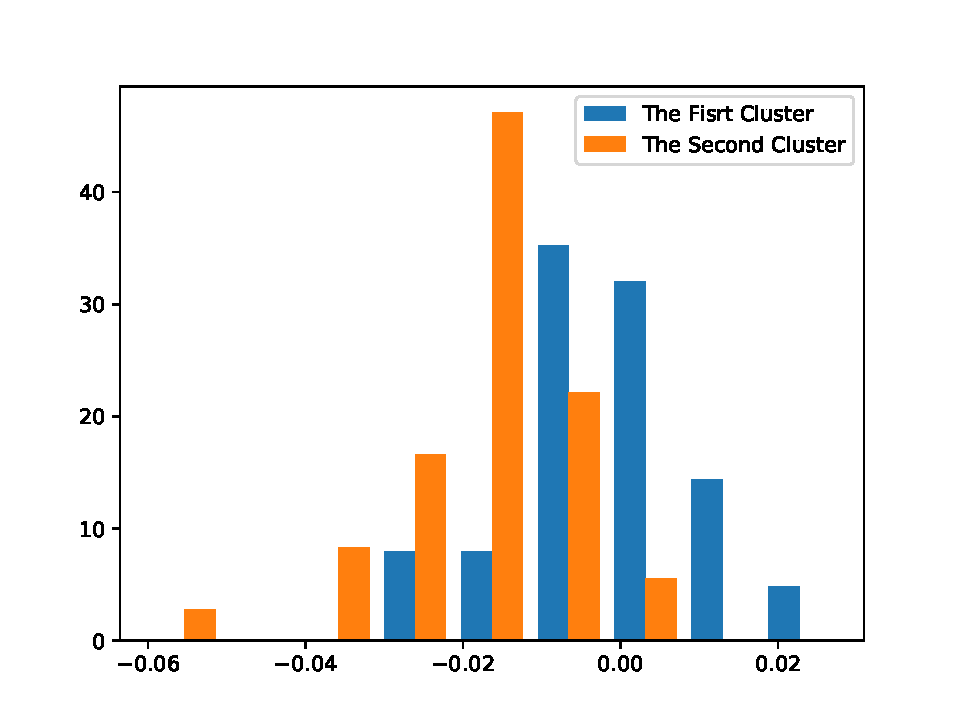
\includegraphics[width=0.4\linewidth]{Images/2.pdf} \label{2} }  
\vspace{2ex}
\subfigure[]{
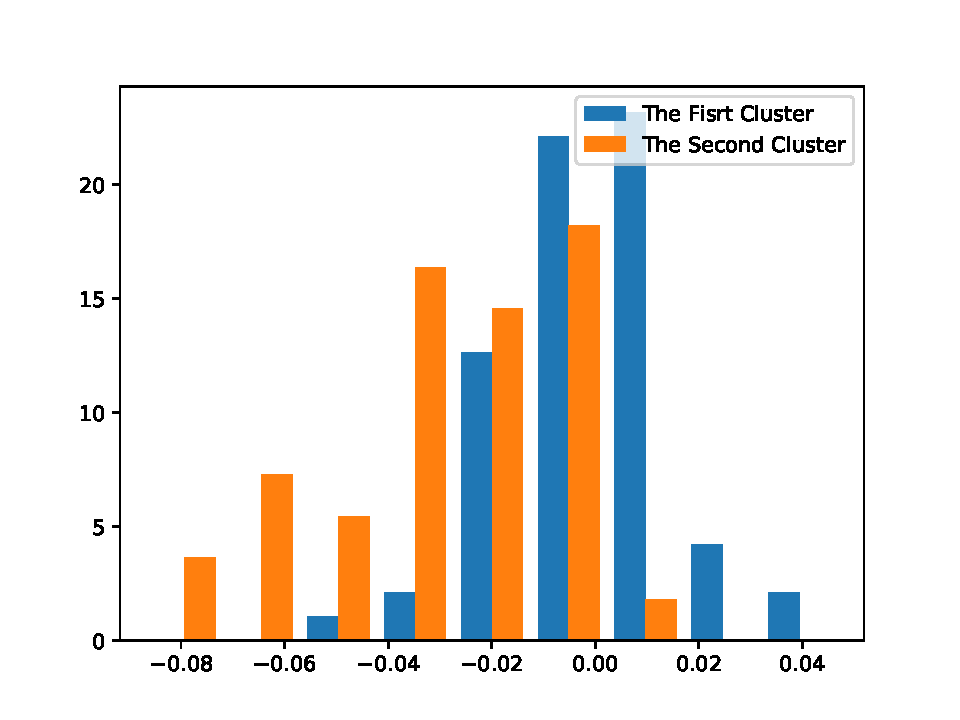
\includegraphics[width=0.4\linewidth]{Images/3.pdf} \label{3} }  
\hspace{2ex}
\subfigure[]{
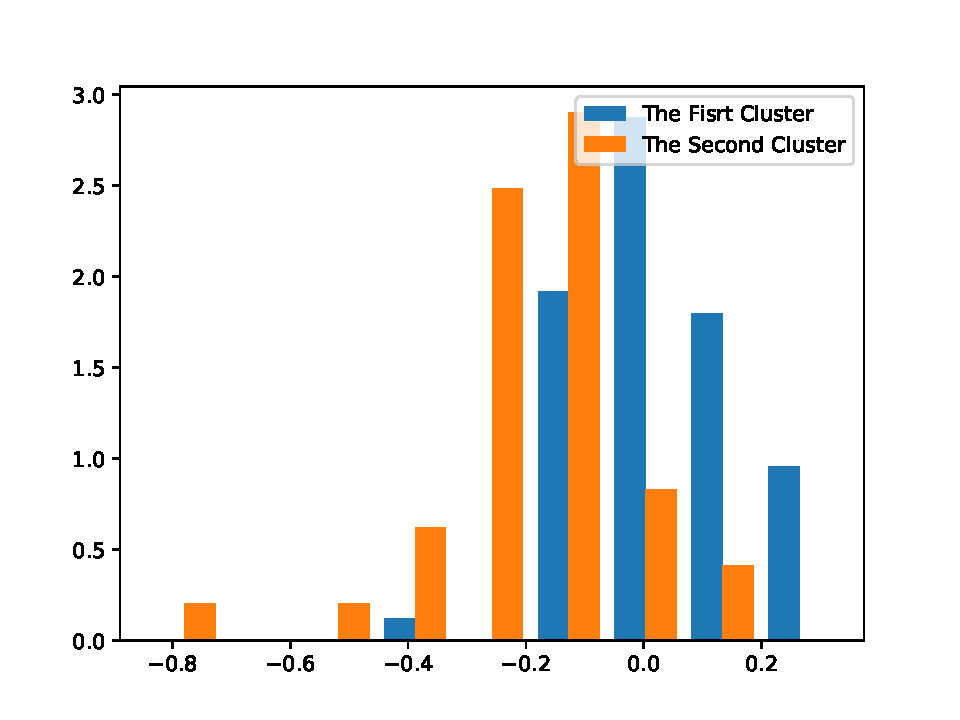
\includegraphics[width=0.4\linewidth]{Images/4.pdf} \label{4} }  
\vspace{2ex}
\subfigure[]{
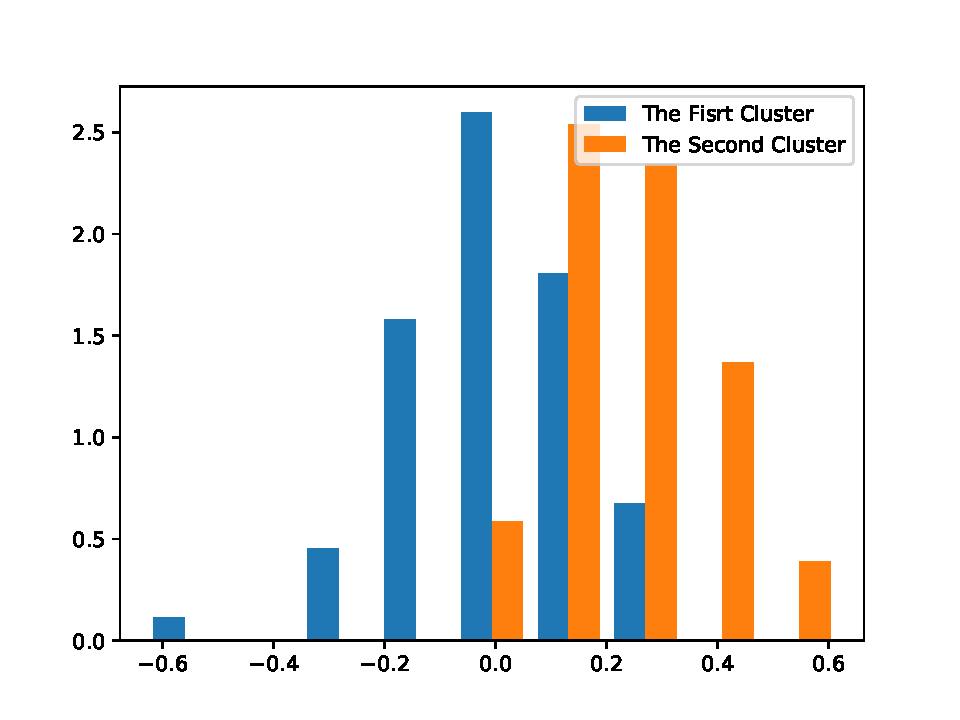
\includegraphics[width=0.4\linewidth]{Images/5.pdf} \label{5} }  
\hspace{2ex}
\subfigure[]{
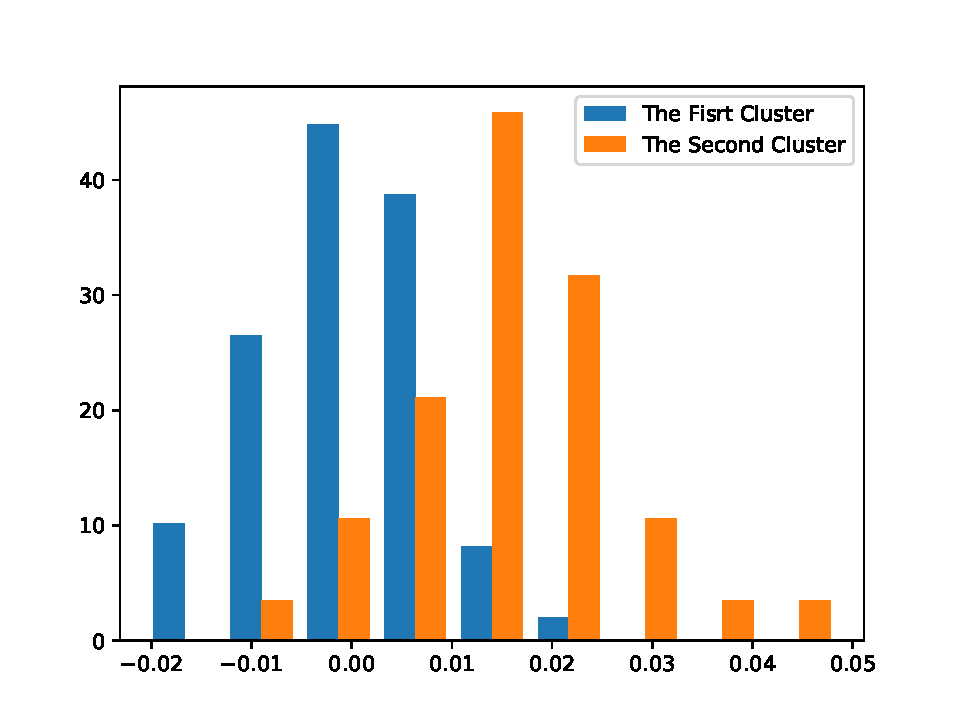
\includegraphics[width=0.4\linewidth]{Images/6.pdf} \label{6} }  

\caption{Сравненение распределения для наиболее различающихся признаков: \subref{1} Доля глаголов прошедшего времени, первого лица, единственного числа; \subref{2} Часть речи: прилагательное; \subref{3} Часть речи: существительное; \subref{4} Средняя длина слов (в количестве символов); \subref{5} Коэффициент Трейгера; \subref{6} Часть речи: местоимение-существительное.} \label{hist}
\end{figure}

\end{document}


